\documentclass[]{article}
\usepackage{lmodern}
\usepackage{amssymb,amsmath}
\usepackage{ifxetex,ifluatex}
\usepackage{fixltx2e} % provides \textsubscript
\ifnum 0\ifxetex 1\fi\ifluatex 1\fi=0 % if pdftex
  \usepackage[T1]{fontenc}
  \usepackage[utf8]{inputenc}
\else % if luatex or xelatex
  \ifxetex
    \usepackage{mathspec}
  \else
    \usepackage{fontspec}
  \fi
  \defaultfontfeatures{Ligatures=TeX,Scale=MatchLowercase}
\fi
% use upquote if available, for straight quotes in verbatim environments
\IfFileExists{upquote.sty}{\usepackage{upquote}}{}
% use microtype if available
\IfFileExists{microtype.sty}{%
\usepackage{microtype}
\UseMicrotypeSet[protrusion]{basicmath} % disable protrusion for tt fonts
}{}
\usepackage[margin=0.25in]{geometry}
\usepackage{hyperref}
\hypersetup{unicode=true,
            pdftitle={lab\_stat565\_1},
            pdfauthor={Shen},
            pdfborder={0 0 0},
            breaklinks=true}
\urlstyle{same}  % don't use monospace font for urls
\usepackage{graphicx,grffile}
\makeatletter
\def\maxwidth{\ifdim\Gin@nat@width>\linewidth\linewidth\else\Gin@nat@width\fi}
\def\maxheight{\ifdim\Gin@nat@height>\textheight\textheight\else\Gin@nat@height\fi}
\makeatother
% Scale images if necessary, so that they will not overflow the page
% margins by default, and it is still possible to overwrite the defaults
% using explicit options in \includegraphics[width, height, ...]{}
\setkeys{Gin}{width=\maxwidth,height=\maxheight,keepaspectratio}
\IfFileExists{parskip.sty}{%
\usepackage{parskip}
}{% else
\setlength{\parindent}{0pt}
\setlength{\parskip}{6pt plus 2pt minus 1pt}
}
\setlength{\emergencystretch}{3em}  % prevent overfull lines
\providecommand{\tightlist}{%
  \setlength{\itemsep}{0pt}\setlength{\parskip}{0pt}}
\setcounter{secnumdepth}{0}
% Redefines (sub)paragraphs to behave more like sections
\ifx\paragraph\undefined\else
\let\oldparagraph\paragraph
\renewcommand{\paragraph}[1]{\oldparagraph{#1}\mbox{}}
\fi
\ifx\subparagraph\undefined\else
\let\oldsubparagraph\subparagraph
\renewcommand{\subparagraph}[1]{\oldsubparagraph{#1}\mbox{}}
\fi

%%% Use protect on footnotes to avoid problems with footnotes in titles
\let\rmarkdownfootnote\footnote%
\def\footnote{\protect\rmarkdownfootnote}

%%% Change title format to be more compact
\usepackage{titling}

% Create subtitle command for use in maketitle
\newcommand{\subtitle}[1]{
  \posttitle{
    \begin{center}\large#1\end{center}
    }
}

\setlength{\droptitle}{-2em}

  \title{lab\_stat565\_1}
    \pretitle{\vspace{\droptitle}\centering\huge}
  \posttitle{\par}
    \author{Shen}
    \preauthor{\centering\large\emph}
  \postauthor{\par}
      \predate{\centering\large\emph}
  \postdate{\par}
    \date{March 08, 2019}


\begin{document}
\maketitle

\begin{enumerate}
\def\labelenumi{(\alph{enumi})}
\tightlist
\item
  Plot the data and report the plot here (A plot with data and means of
  treatment combinations). Do not report code here. Describe the
  observed relationship between two factors.
\end{enumerate}

\begin{verbatim}
## Observations: 40
## Variables: 3
## $ Source <chr> "Beef", "Beef", "Beef", "Beef", "Beef", "Beef", "Beef",...
## $ Amount <chr> "Low", "Low", "Low", "Low", "Low", "Low", "Low", "Low",...
## $ Gain   <dbl> 90, 76, 90, 64, 86, 51, 72, 90, 95, 78, 73, 102, 118, 1...
\end{verbatim}

\begin{verbatim}
## Observations: 40
## Variables: 3
## $ Source <chr> "Beef", "Beef", "Beef", "Beef", "Beef", "Beef", "Beef",...
## $ Amount <chr> "Low", "Low", "Low", "Low", "Low", "Low", "Low", "Low",...
## $ Gain   <dbl> 90, 76, 90, 64, 86, 51, 72, 90, 95, 78, 73, 102, 118, 1...
\end{verbatim}

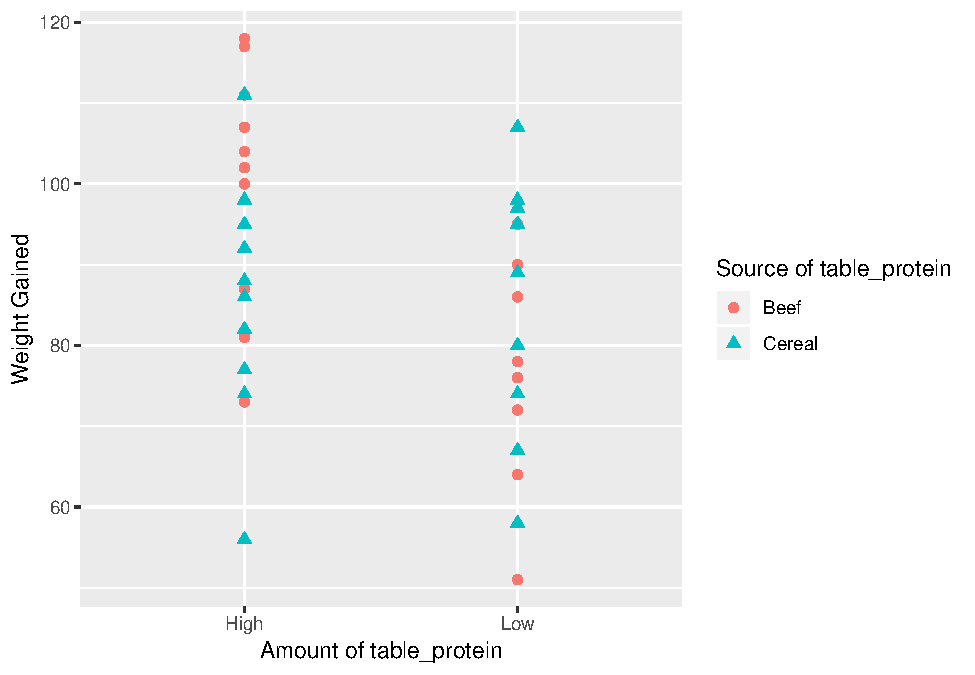
\includegraphics[width=0.25\linewidth]{lab_stat565_1_files/figure-latex/pressure-1}

\begin{verbatim}
## No summary function supplied, defaulting to `mean_se()
\end{verbatim}

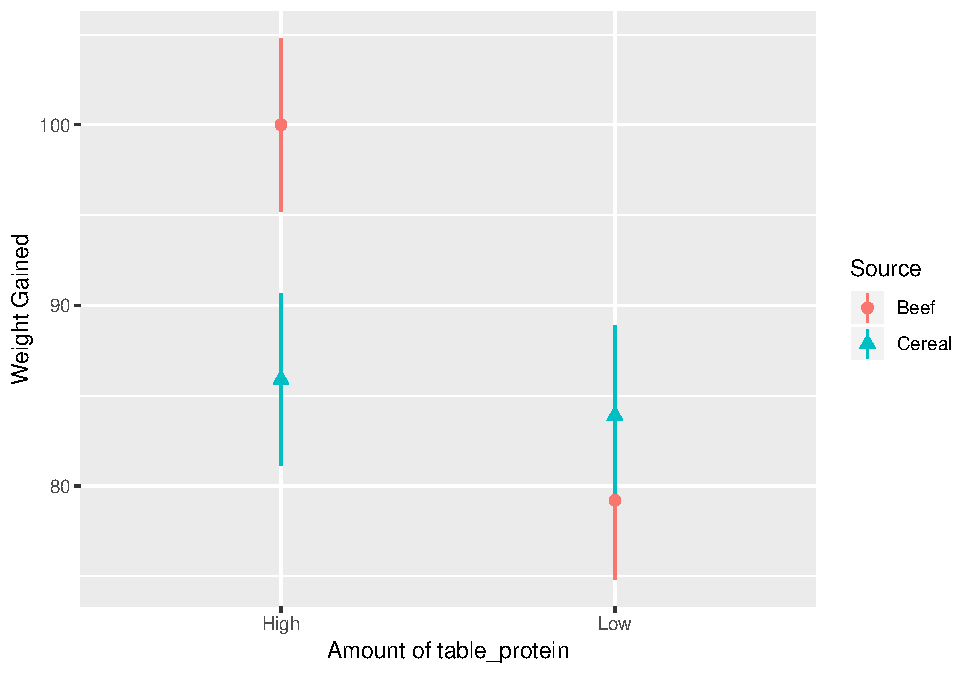
\includegraphics[width=0.25\linewidth]{lab_stat565_1_files/figure-latex/pressure-2}
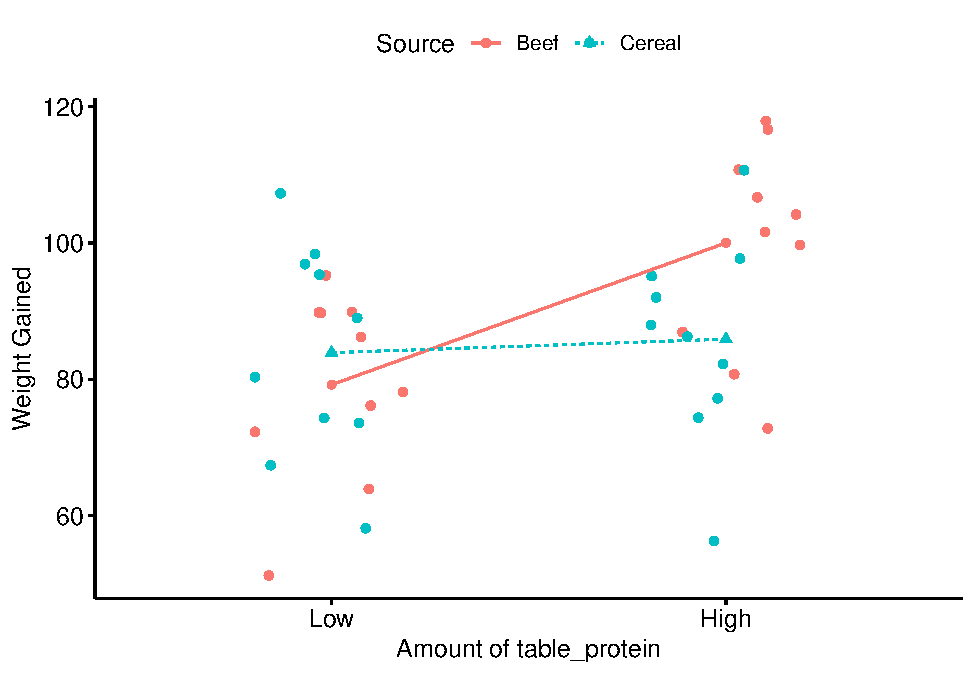
\includegraphics[width=0.25\linewidth]{lab_stat565_1_files/figure-latex/pressure-3}

\begin{verbatim}
##   Source min   Q1 median    Q3 max mean       sd  n missing
## 1   Beef  51 77.5     90 102.5 118 89.6 17.71232 20       0
## 2 Cereal  56 74.0     87  95.5 111 84.9 14.99438 20       0
##   Amount min    Q1 median     Q3 max  mean       sd  n missing
## 1   High  56 81.75   93.5 104.75 118 92.95 16.36259 20       0
## 2    Low  51 73.50   83.0  91.25 107 81.55 14.63045 20       0
##        Amount min    Q1 median     Q3 max   mean       sd  n missing
## 1   Beef.High  73 90.25  103.0 110.00 118 100.00 15.13642 10       0
## 2 Cereal.High  56 78.25   87.0  94.25 111  85.90 15.02184 10       0
## 3    Beef.Low  51 73.00   82.0  90.00  95  79.20 13.88684 10       0
## 4  Cereal.Low  58 74.00   84.5  96.50 107  83.90 15.70881 10       0
## 5        High  56 81.75   93.5 104.75 118  92.95 16.36259 20       0
## 6         Low  51 73.50   83.0  91.25 107  81.55 14.63045 20       0
##             Df Sum Sq Mean Sq F value Pr(>F)  
## Trt1         1    221   220.9   0.988 0.3269  
## Trt2         1   1300  1299.6   5.812 0.0211 *
## Trt1:Trt2    1    884   883.6   3.952 0.0545 .
## Residuals   36   8049   223.6                 
## ---
## Signif. codes:  0 '***' 0.001 '**' 0.01 '*' 0.05 '.' 0.1 ' ' 1
\end{verbatim}

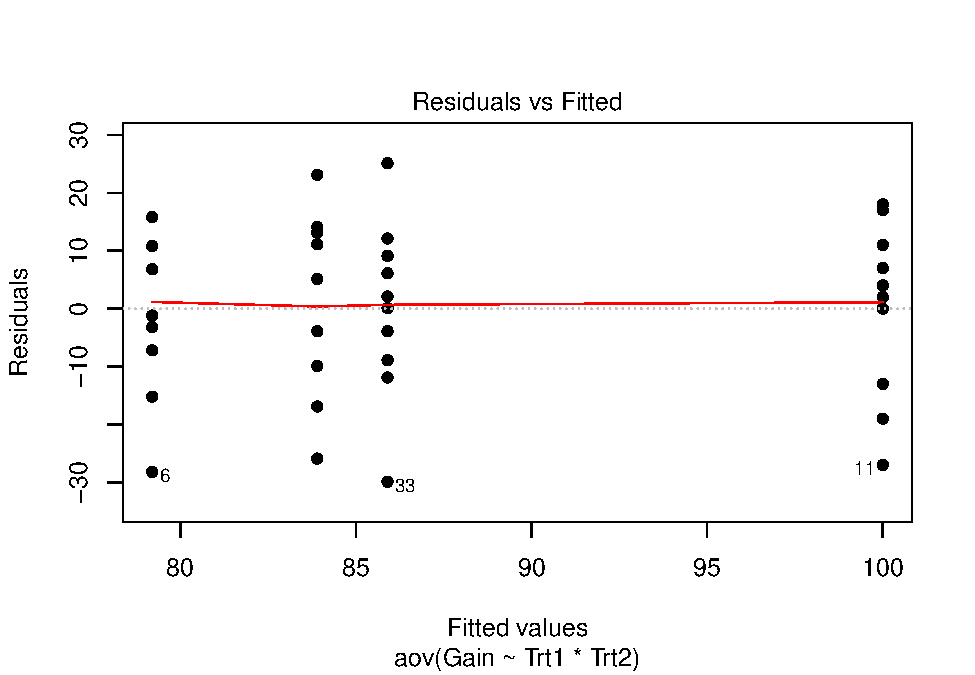
\includegraphics[width=0.25\linewidth]{lab_stat565_1_files/figure-latex/pressure-4}
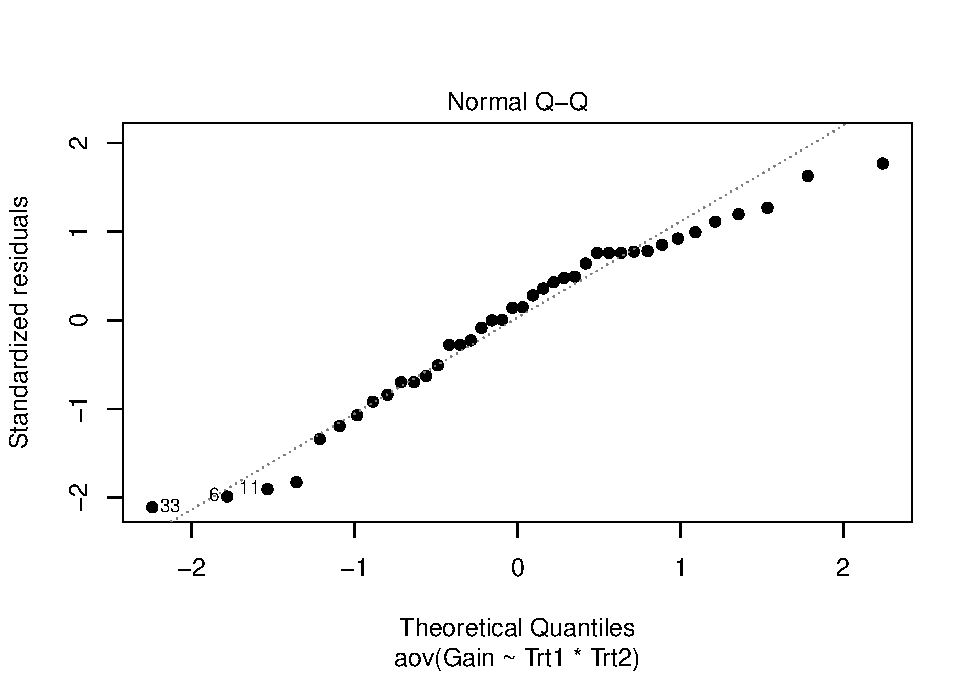
\includegraphics[width=0.25\linewidth]{lab_stat565_1_files/figure-latex/pressure-5}
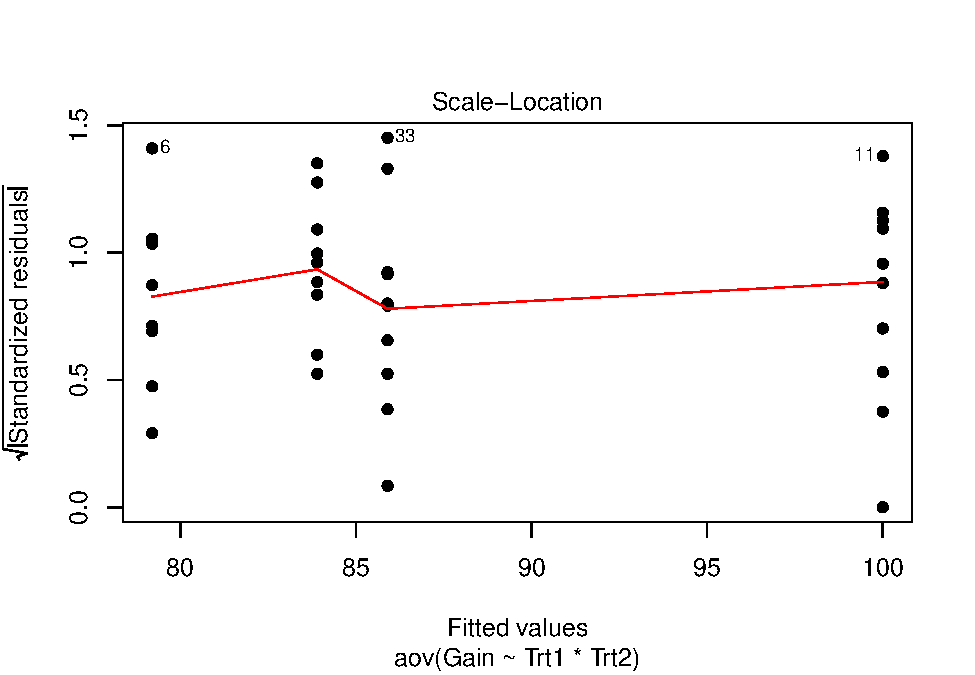
\includegraphics[width=0.25\linewidth]{lab_stat565_1_files/figure-latex/pressure-6}
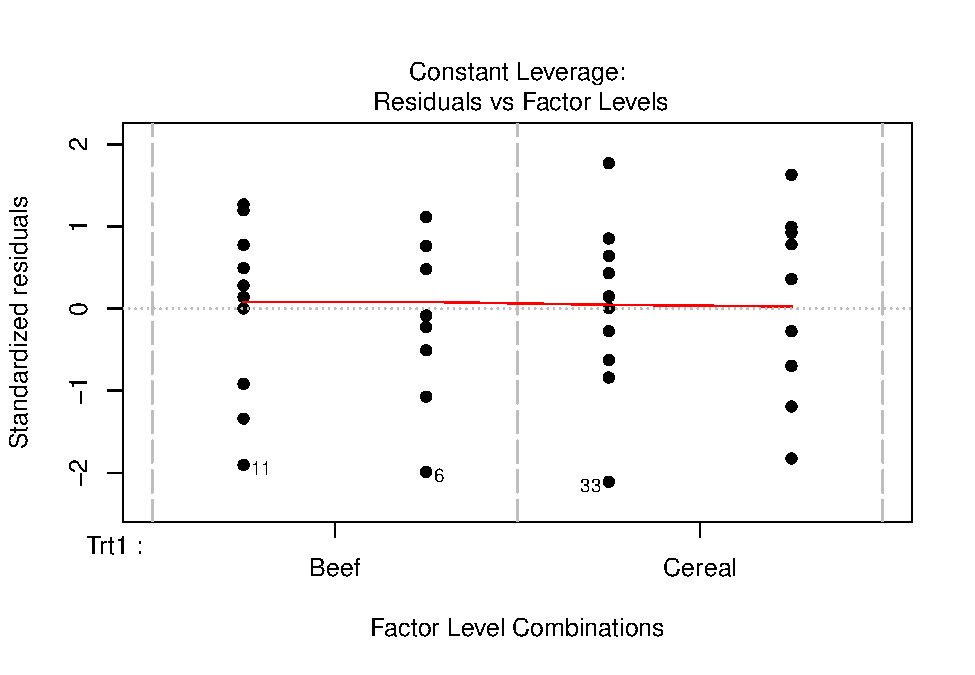
\includegraphics[width=0.25\linewidth]{lab_stat565_1_files/figure-latex/pressure-7}

\begin{verbatim}
## 
##  Pairwise comparisons using t tests with pooled SD 
## 
## data:  table_protein$Gain and table_protein$Trt2 
## 
##     High 
## Low 0.026
## 
## P value adjustment method: none
## 
##  Pairwise comparisons using t tests with pooled SD 
## 
## data:  table_protein$Gain and table_protein$Trt2 
## 
##     High 
## Low 0.026
## 
## P value adjustment method: bonferroni
\end{verbatim}

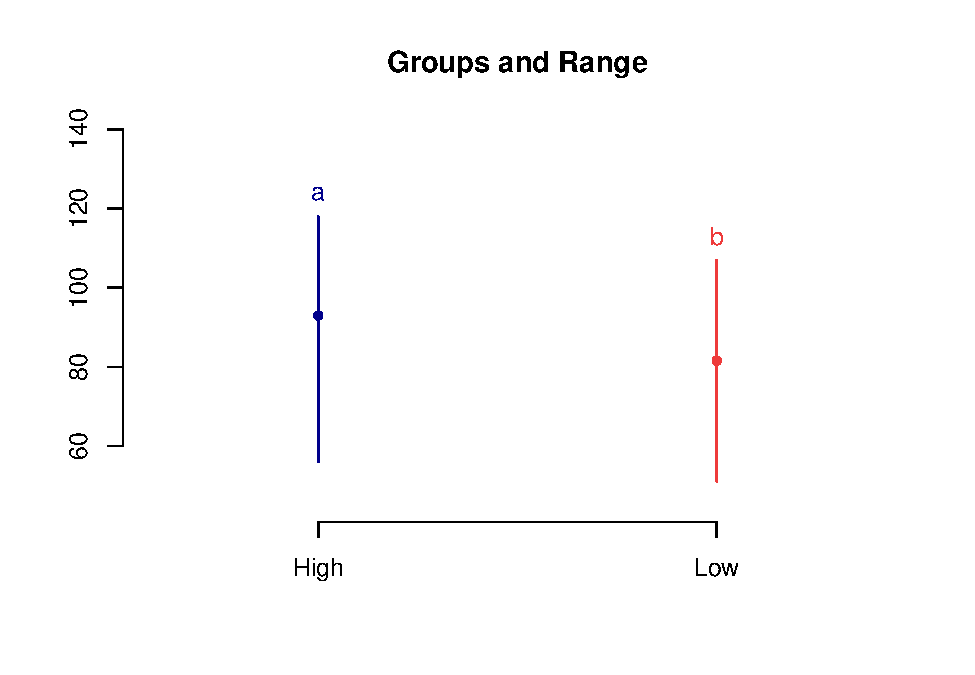
\includegraphics[width=0.25\linewidth]{lab_stat565_1_files/figure-latex/pressure-8}

\begin{verbatim}
## $statistics
##    MSerror Df  Mean       CV  t.value  LSD
##   223.5944 36 87.25 17.13819 2.028094 9.59
## 
## $parameters
##         test p.ajusted name.t ntr alpha
##   Fisher-LSD      none   Trt2   2  0.05
## 
## $means
##       Gain      std  r      LCL      UCL Min Max   Q25  Q50    Q75
## High 92.95 16.36259 20 86.16885 99.73115  56 118 81.75 93.5 104.75
## Low  81.55 14.63045 20 74.76885 88.33115  51 107 73.50 83.0  91.25
## 
## $comparison
## NULL
## 
## $groups
##       Gain groups
## High 92.95      a
## Low  81.55      b
## 
## attr(,"class")
## [1] "group"
##   Tukey multiple comparisons of means
##     95% family-wise confidence level
## 
## Fit: aov(formula = Gain ~ Trt1 * Trt2, data = table_protein)
## 
## $Trt1
##             diff    lwr  upr     p adj
## Cereal-Beef -4.7 -14.29 4.89 0.3268783
## 
## $Trt2
##           diff    lwr   upr     p adj
## Low-High -11.4 -20.99 -1.81 0.0211449
## 
## $`Trt1:Trt2`
##                         diff      lwr       upr     p adj
## Cereal:High-Beef:High  -14.1 -32.1102  3.910198 0.1697711
## Beef:Low-Beef:High     -20.8 -38.8102 -2.789802 0.0182745
## Cereal:Low-Beef:High   -16.1 -34.1102  1.910198 0.0936982
## Beef:Low-Cereal:High    -6.7 -24.7102 11.310198 0.7492577
## Cereal:Low-Cereal:High  -2.0 -20.0102 16.010198 0.9905411
## Cereal:Low-Beef:Low      4.7 -13.3102 22.710198 0.8952934
## 
##   Posthoc multiple comparisons of means : Scheffe Test 
##     95% family-wise confidence level
## 
## $Trt1
##             diff    lwr.ci   upr.ci   pval    
## Cereal-Beef -4.7 -18.56594 9.165941 0.8042    
## 
## $Trt2
##           diff    lwr.ci   upr.ci   pval    
## Low-High -11.4 -25.26594 2.465941 0.1410    
## 
## $`Trt1:Trt2`
##                         diff   lwr.ci    upr.ci   pval    
## Cereal:High-Beef:High  -14.1 -33.7094  5.509402 0.2358    
## Beef:Low-Beef:High     -20.8 -40.4094 -1.190598 0.0338 *  
## Cereal:Low-Beef:High   -16.1 -35.7094  3.509402 0.1418    
## Beef:Low-Cereal:High    -6.7 -26.3094 12.909402 0.8004    
## Cereal:Low-Cereal:High  -2.0 -21.6094 17.609402 0.9929    
## Cereal:Low-Beef:Low      4.7 -14.9094 24.309402 0.9195    
## 
## ---
## Signif. codes:  0 '***' 0.001 '**' 0.01 '*' 0.05 '.' 0.1 ' ' 1
\end{verbatim}


\end{document}
